\documentclass{beamer}
\usepackage{graphicx, parskip, microtype}

\frenchspacing

\usetheme{default}
\usecolortheme{whale}

\setbeamertemplate{navigation symbols}{}

\setbeamercolor{title}{fg=blue,bg=white}

\setbeamercolor{block title}{fg=white,bg=gray}
\setbeamercolor{block body}{fg=black,bg=lightgray}

\setbeamercolor{block title alerted}{fg=white,bg=darkgray}
\setbeamercolor{block body alerted}{fg=black,bg=lightgray}

\title{From the bottom of the wiki hole}
\author{Peter D Smits}
\institute{Committee on Evolutionary Biology, University of Chicago}

\begin{document}

\begin{frame}
  \maketitle
\end{frame}

\begin{frame}
  \frametitle{or\dots}
  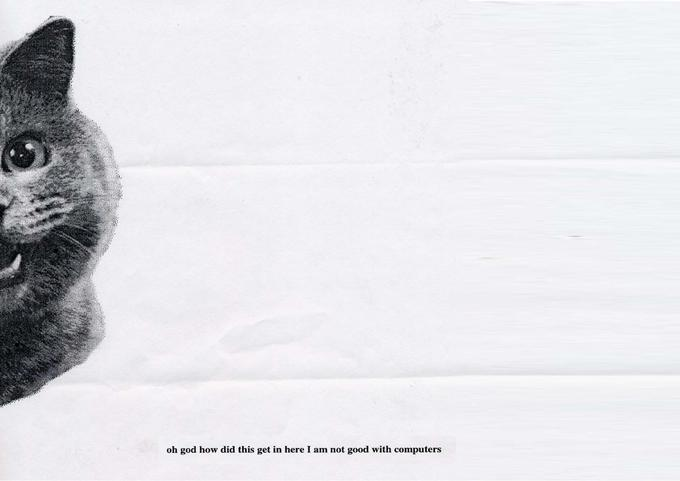
\includegraphics[width = \textwidth, keepaspectratio = true]{figure/happy_cat}
\end{frame}

\begin{frame}
  \frametitle{What?}
  \begin{center}
    
\includegraphics[height = 0.8\textheight, keepaspectratio = true]{figure/wiki}
  \end{center}
\end{frame}

\begin{frame}
  \frametitle{How many?}
  \begin{center}
    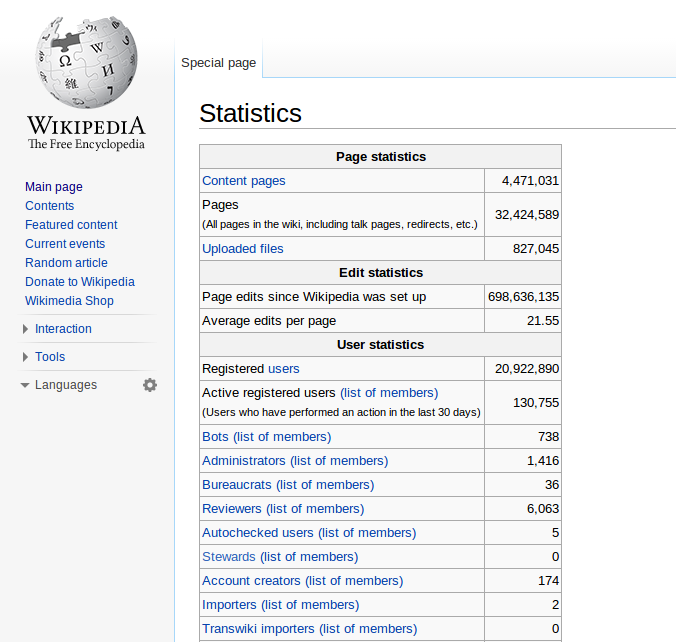
\includegraphics[height = 0.8\textheight, keepaspectratio = true]{figure/wiki_stats}
  \end{center}
\end{frame}

\begin{frame}
  \frametitle{Who?}
  \begin{center}
    
\includegraphics[height = 0.8\textheight, keepaspectratio = true]{figure/wiki_family}
  \end{center}
\end{frame}

\begin{frame}
  \frametitle{Problems? In my wiki?}
  \begin{center}
    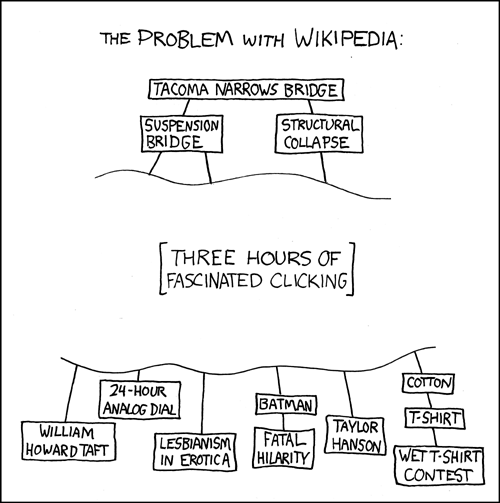
\includegraphics[height = 0.8\textheight, keepaspectratio = true]{figure/the_problem_with_wikipedia}
  \end{center}
\end{frame}

\begin{frame}
  \frametitle{Oh no pigeons}
  \begin{center}
    
\includegraphics[width = \textwidth, keepaspectratio = true]{figure/wiki_game}
  \end{center}
\end{frame}

\begin{frame}
  \frametitle{There is more than one wiki?}
  \begin{center}
    
\includegraphics[width = \textwidth, keepaspectratio = true]{figure/wikia}
  \end{center}
\end{frame}

\begin{frame}
  \frametitle{wiki-ing intensifies}
  \begin{center}
    \noindent
    
\includegraphics[width = 0.3\textwidth, keepaspectratio = true]{figure/tropes}\hspace{0.2\textwidth}
    
\includegraphics[width = 0.4\textwidth, height = 0.4\textheight, keepaspectratio = true]{figure/memalpha1}\\[2em]
    
\includegraphics[width = 0.4\textwidth, height = 0.4\textheight, keepaspectratio = true]{figure/wookie}\hspace{0.2\textwidth}
    
\includegraphics[width = 0.4\textwidth, height = 0.4\textheight, keepaspectratio = true]{figure/bulbapedia}\par
  \end{center}
\end{frame}

\begin{frame}
  \frametitle{heavy breathing}
  \begin{center}
    
\includegraphics[width = \textwidth, keepaspectratio = true]{figure/ice}

    
\includegraphics[width = 0.6\textwidth, keepaspectratio = true]{figure/got}
  \end{center}
\end{frame}

\begin{frame}
  \frametitle{Niche projects?}
  \begin{columns}
    \begin{column}{0.5\textwidth}
      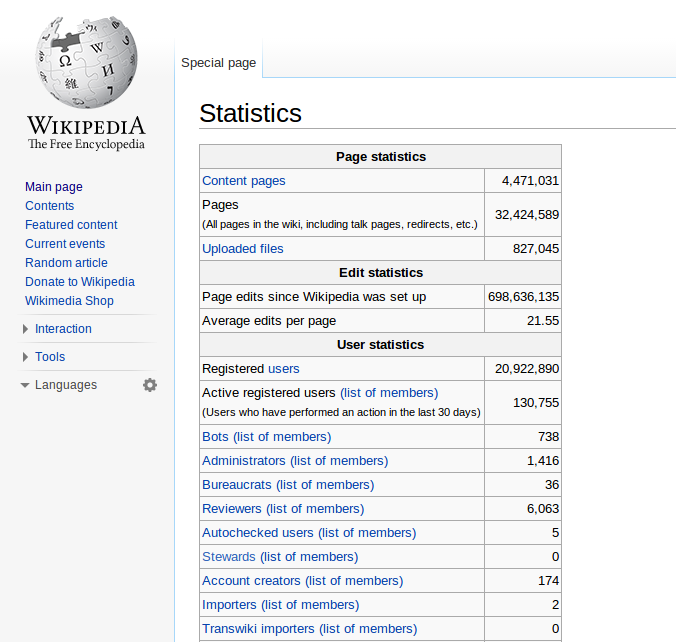
\includegraphics[height = 0.8\textheight, width = \textwidth, keepaspectratio = true]{figure/wiki_stats}
    \end{column}
    \begin{column}{0.5\textwidth}
      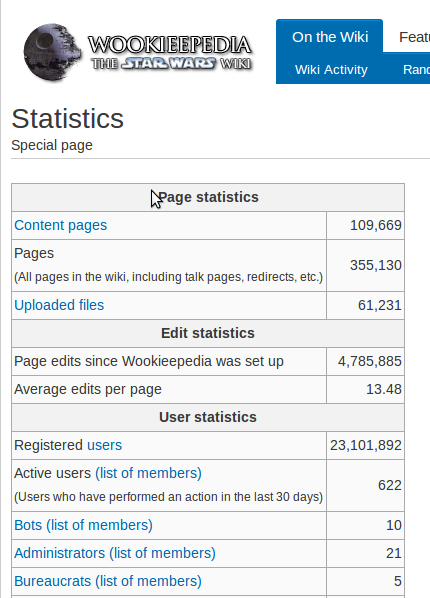
\includegraphics[height = 0.8\textheight, width = \textwidth, keepaspectratio = true]{figure/wookie_stats}
    \end{column}
  \end{columns}
\end{frame}

\begin{frame}
  \frametitle{Niche projects?}
  \begin{columns}
    \begin{column}{0.5\textwidth}
      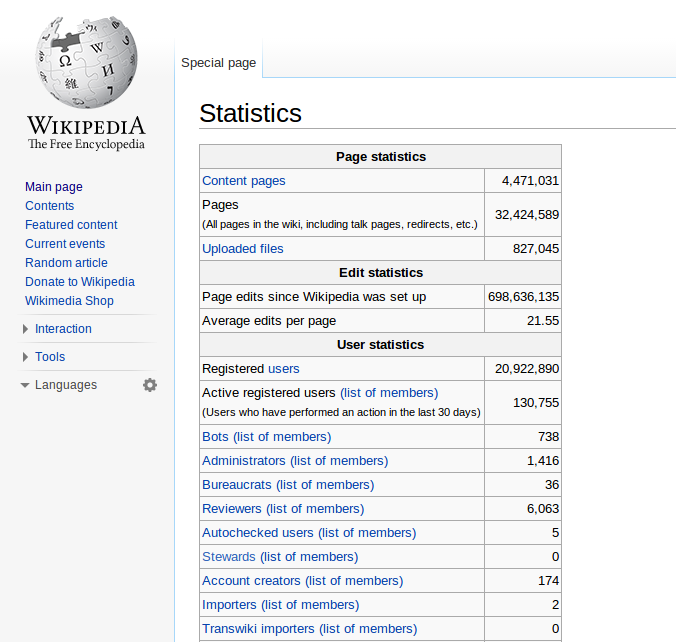
\includegraphics[height = 0.8\textheight, width = \textwidth, keepaspectratio = true]{figure/wiki_stats}
    \end{column}
    \begin{column}{0.5\textwidth}
      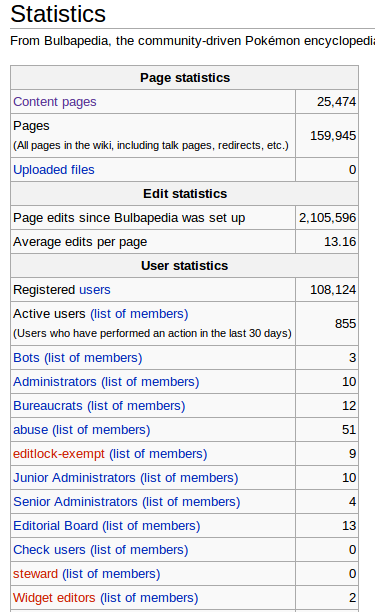
\includegraphics[height = 0.8\textheight, width = \textwidth, keepaspectratio = true]{figure/bulb_stats}
    \end{column}
  \end{columns}
\end{frame}

\begin{frame}
  \frametitle{Niche projects?}
  \begin{columns}
    \begin{column}{0.5\textwidth}
      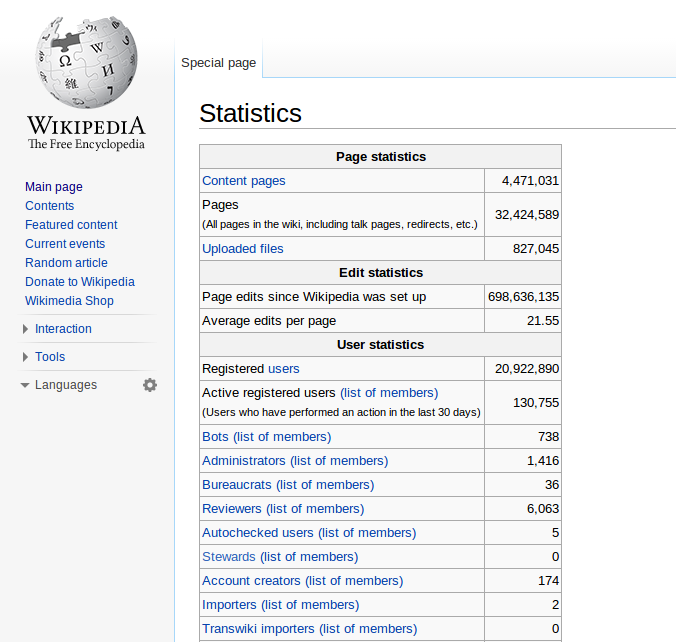
\includegraphics[height = 0.8\textheight, width = \textwidth, keepaspectratio = true]{figure/wiki_stats}
    \end{column}
    \begin{column}{0.5\textwidth}
      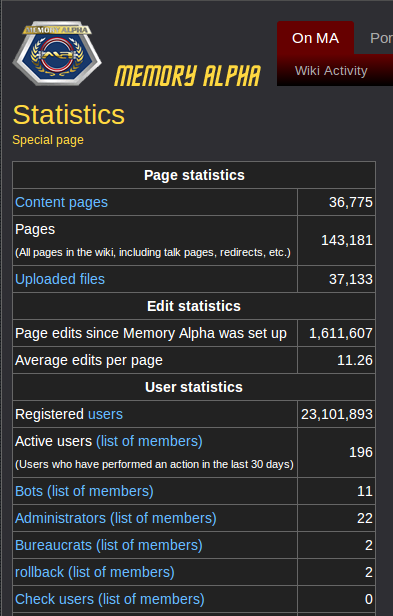
\includegraphics[height = 0.8\textheight, width = \textwidth, keepaspectratio = true]{figure/trek_stats}
    \end{column}
  \end{columns}
\end{frame}

\begin{frame}
  \frametitle{Analysis time!}
  \begin{columns}
    \begin{column}{0.5\textwidth}
      
\includegraphics[width = \textwidth, keepaspectratio = true]{figure/tos}

      
\includegraphics[width = \textwidth, keepaspectratio = true]{figure/ds9}
    \end{column}
    \begin{column}{0.5\textwidth}
      
\includegraphics[width = \textwidth, keepaspectratio = true]{figure/tng}

      
\includegraphics[width = \textwidth, keepaspectratio = true]{figure/voy}
    \end{column}
  \end{columns}
\end{frame}

\begin{frame}
  \frametitle{tl;dr}
  \begin{itemize}
    \item memory alpha dump
      \begin{itemize}
        \item XML format
        \item every, and i mean every, current page
        \item no images
        \item \~{} 313 MB
      \end{itemize}
    \item R plus packages
      \begin{itemize}
        \item see what you can do with your degree?
      \end{itemize}
    \item link network. content pages. both in and out of universe.
  \end{itemize}
\end{frame}

\begin{frame}
  \frametitle{Questions}
  \huge{Captains? (and commander\ldots )}

  \huge{Series?}
  
  \huge{Episodes?}

  \huge{etc.}
\end{frame}

\begin{frame}
  \frametitle{summaries}
\end{frame}

\begin{frame}
  \frametitle{captains}
  % image & value
  % reveal with clicks
\end{frame}

\begin{frame}
  \frametitle{series}
  % image & value
  % reveal with clicks
\end{frame}

\begin{frame}
  \frametitle{episodes}
  % image & value
  % reveal with clicks
\end{frame}

\begin{frame}
  \frametitle{10 most important ``things''}
  % reveal with clicks
\end{frame}

\begin{frame}
  \frametitle{emergent structure?}
  % graph plot with communities as nodes, vertex size based on number of nodes inside
\end{frame}


\end{document}
